\chapter{Design}
In this chapter, we define the Turing Machine Language (TML) as an alternative to Turing Machines (TM). We will define the syntax of a TML program and how it can be executed on a tape in a similar manner to TMs. We will then prove that there is an equivalence between TML programs and TMs in terms of their execution on a tape.

\section{Turing Machine Language Program}
In this section, we will define the syntax of the Turing Machine Language with an example. We next analyse the syntax and define execution of a valid TML program on a tape in a similar manner to the execution of a TM.

Consider the following TML program.
\begin{lstlisting}[language=TML]
alphabet = {"0", "1"}
module isEven {
    switch tapehead {
        while 0, 1 {
            move right
        } if blank {
            move left
            switch tapehead {
                if 0 {
                    changeto blank
                    accept
                } if 1, blank {
                    changeto blank
                    reject
                }
            }
        }
    }
}
\end{lstlisting}
A program in TML will be used to execute on a tape, so the syntax used guides us in executing the program on a tape. We will see that later. For now, we consider the rules of the TML program:
\begin{itemize}
    \item A valid TML \emph{program} is composed of the \emph{alphabet}, followed by one or more \emph{modules}. In the example above, the alphabet of the program is $\{0, 1\}$, and the program has a single module called \texttt{isEven}.
    \item A module contains one or more \emph{blocks} (a specific sequence of commands). There are two types of blocks- \emph{basic blocks} and \emph{switch blocks}.
    \item A basic block consists of \emph{basic commands} (\textit{changeto}, \textit{move} or \textit{flow} command). A basic block consists of at least one basic command, but it is not necessary for a basic block to be composed of all the basic commands. If multiple commands are present in a basic block, they must be in the following order- \textit{changeto}, \textit{move} and \textit{flow} command. In the program above, there is are many basic blocks, e.g. at lines 5, 7, 10-11 and 13-14. We do not say that line 10 is a basic block by itself; we want the basic block to be as long as possible.
    \item A \emph{switch block} consists of a single switch statement. A switch statement must contain precisely one case (\textit{if} or \textit{while} command) for each of the letter in the alphabet, including the \texttt{blank} letter. The first block of a case block must be a basic block. In the program above, there is a switch block at lines 8-16.
    \item The body of an \textit{if} command can be composed of multiple blocks. These blocks can be both basic blocks and switch blocks. We can see this at lines 6-17; the \textit{if} block has a basic block at line 7 and then a switch block.
    \item The body of a \textit{while} command must be composed of a single basic block. The basic block cannot have a \textit{flow} command. This is because when we execute a \textit{while} block, the next block to run is the switch block it is in; we cannot accept, reject or go to another module.
    \item A switch block must be the final block present; it cannot be followed by any other block, basic or switch.
\end{itemize}
The EBNF for the TML and examples of syntax errors are given in the appendix. 

We will now consider how to execute a tape on a valid TML program. Let $P$ be a TML program with alphabet $\Sigma$ and let $T$ be a tape on $\Sigma$. We execute $P$ on $T$ inductively, as follows:
\begin{itemize}
    \item At any point during execution, we maintain 3 objects- a tape on $\Sigma$, a block of $P$ and the tapehead index. 
    \item At the start, the tape is $T$; the tapehead index is $0$; and the block is the first block in the first module in $P$. 
    \item At some point during the execution, assume that we have the tape $S$, tapehead index $j$, with tapehead value $T(j) = t$, and a block $b$. We define the next triple as follows:
    \begin{itemize}
        \item if $b$ is a switch block, we take the first block from the case corresponding to the tapehead value- because the program is valid, this is a basic block; we will now refer to this block as $b$.
        \item if $b$ has a \textit{changeto} \texttt{val} command, the next tape $T'$ is given by 
        \[T'(x) = \begin{cases}
            \texttt{val} & x = i \\
            T(x) & \text{otherwise}.
        \end{cases}\]
        If the \textit{changeto} command is missing, then the tapehead $T' = T$.
        \item if $b$ has a \textit{move} \texttt{dir} command, the next tapehead index is given by:
        \[i' = \begin{cases}
            i+1 & \texttt{dir} = \texttt{right} \\
            i-1 & \texttt{dir} = \texttt{left}.
        \end{cases}\]
        If the \textit{move} command is missing, then $i' = i-1$.
        \item we either terminate or determine the next block $b'$ to execute (in decreasing precedence):
        \begin{itemize}
            \item if the block is the body of a while case block, then the next block $b' = b$, i.e. we execute this switch block again (not necessarily the same case block);
            \item if the block contains a terminating \textit{flow} command, execution is terminated and we return the terminated state (\texttt{accept} or \texttt{reject});
            \item if the block contains a \textit{goto} \texttt{mod} command, then $b'$ is the first block of the module \texttt{mod};
            \item if the block is not the final block in the current module, then $b'$ is next block in this module;
            \item otherwise, execution is terminated and we return the state \texttt{reject}.
        \end{itemize}
    \end{itemize}
    If execution is not terminated, execution continues with the next triplet.
\end{itemize}
An example that illustrates the execution process is given in the appendix.

\section{Complete TML Programs}
When we defined execution of a valid TML program on a tape above, we said that a basic block need not have all 3 types of commands (\textit{changeto}, \textit{move} and a \textit{flow} command), but in the execution above, we have established some `default' ways in which a program gets executed. In particular,
\begin{itemize}
    \item if the \textit{changeto} command is missing, we do not change the value of the tape;
    \item if the \textit{move} command is missing, we move left;
    \item if the \textit{flow} command is missing, we can establish what to do using the rules described above- this is a bit more complicated than the two commands above.
\end{itemize}
Nonetheless, it is possible to include these `default' commands to give a \emph{complete} version of the program. This is what we will establish in this section. 

Consider the following complete program.
\begin{lstlisting}[language=TML]
alphabet = {"0", "1"}
module isOdd {
    // move to the end
    switch tapehead {
        while 0 {
            changeto 0
            move right
        } while 1 {
            changeto 1
            move right
        } if blank {
            changeto blank
            move left
            goto isOddCheck
        }
    }
}
module isOddCheck {
    // accept if and only if the value is 1
    switch tapehead {
        if 0, blank {
            changeto 0
            move left
            reject
        } if 1 {
            changeto blank
            move left
            accept
        }
    }
}
\end{lstlisting}
Now, we consider the rules that a complete TML program obeys:
\begin{itemize}
    \item A basic block in a complete program has all the necessary commands- if the basic block is inside \textit{while} case, it has a \textit{changeto} command and a \textit{move} command; otherwise, it also has a \textit{flow} command.
    \item A module in a complete program is composed of a single switch block.
\end{itemize}

% By adding the `default' values for the \textit{changeto} and the \textit{move} command, we can partly complete a valid TML program. We can further break 
We will now construct a complete TML program for a valid TML program.
\begin{enumerate}
    \item We first break each module into smaller modules so that every module has just one basic/switch block- we add a \textit{goto} command to the next module if it appeared just below this block.
    \item Then, we can convert each basic block to a switch block by just adding a single case that applies to each letter in the alphabet.
    \item Finally, we add the default values to each basic block to get a complete TML program.
\end{enumerate}
This way, we can associate every block in the valid program with a corresponding block in the complete program. The complete version is always a switch block and might have more commands than the original block, but it still has all the commands present in the original block. 

An example that illustrates this process is given in the appendix.

\begin{theorem}
    Let $P$ be a valid TM program. Then, $P$ and its completion $P^+$ execute on every valid tape $T$ in the same way.
\end{theorem}
The proof of the theorem is given in the appendix.

Because of the equivalence between valid and complete programs, we will assume that every valid program is complete from now on.

\section{Equivalence of TMs and TMLs}
In this section, we will show that there is an equivalence between TMs and valid (complete) TML programs. We will first construct a valid TML program for a TM and then show that it has the same behaviour as the TM. Later, we will construct a TM for a complete TML program, and show the equivalence in this case as well.

We will first illustrate how to convert a TM to a (complete) TML program. So, consider the following TM:
Consider the following TM:
\begin{figure}[H]
    \centering
    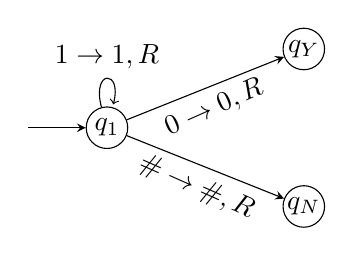
\begin{tikzpicture}
        \node[circle, draw=black, fill=white, inner sep=0pt, minimum size=15pt] (s1) at (2.5, 0) {$q_1$};
        \node[circle, draw=black, fill=white, inner sep=0pt, minimum size=15pt] (sN) at (5, -1) {$q_N$};                
        \node[circle, draw=black, fill=white, inner sep=0pt, minimum size=15pt] (sY) at (5, 1) {$q_Y$};

        \draw[-stealth] (1.5, 0) -- (s1);
        
        \draw[-stealth] (s1) edge[loop above] node[above] {$1 \to 1, R$} (s1);
        
        \draw[-stealth] (s1) -- node[below, rotate=24] {$0 \to 0, R$} (sY);
        \draw[-stealth] (s1) -- node[below, rotate=-24] {$\# \to \#, R$} (sN);
    \end{tikzpicture}
\end{figure}
Then, its corresponding TML program is the following:
\begin{lstlisting}[language=TML]
alphabet = {"0", "1"}
module has0 {
    switch tapehead {
        while 1 {
            changeto 1
            move right
        } if 0 {
            changeto 1
            move right
            accept
        } if blank {
            changeto blank
            move left
            reject
        }
    }
}
\end{lstlisting}
In general, we convert each (non-terminating) state in the TM $M$ to a TML module. The following is how we create the module:
\begin{itemize}
    \item the module contains a single \textit{switch} command;
    \item for each letter $\sigma$ in the alphabet $\Sigma^+$, denote $\delta(q, \sigma) = (q', \sigma', \texttt{dir})$. We add a case in the \textit{switch} command corresponding to letter $\sigma$ (an \textit{if} case if $q' \neq q$, otherwise a \textit{while} case) with the following commands:
    \begin{itemize}
        \item \texttt{changeto} $\sigma'$
        \item \texttt{move} \textit{dir}
        \item in the case of an \textit{if} block, if $q'$ is \texttt{accept}, then the command \texttt{accept}; if $q'$ is \texttt{reject}, then the command \texttt{reject}; otherwise, \texttt{goto} $q'$.
    \end{itemize}
\end{itemize}
Moreover, we can construct the program $P$ with:
\begin{itemize}
    \item the alphabet $\Sigma$;
    \item modules corresponding to every state $q$ in $M$;
    \item the module corresponding to the initial state $q_0$ placed at the top.
\end{itemize}
We say that $P$ is \emph{the corresponding program for $M$}.

\begin{theorem}
    Let $M$ be a TM, and let $P$ be the corresponding program for $M$. Then, $M$ and $P$ execute on every valid tape $T$ in the same way. 
\end{theorem}
The proof of the theorem is given in the appendix.

Next, we construct a TM for a (complete) TML program. This process is essentially the inverse of the one we saw converting a complete TML program to a TM. In particular, for each module $m$ in $P$, we construct the state $q$ as follows- for each letter $\sigma$ in $\Sigma^+$, we define $\delta(q, \sigma) = (q', \sigma', \texttt{dir})$, where:
\begin{itemize}
    \item the value $\sigma'$ is the letter given in the \textit{changeto} command within $m$;
    \item the value \texttt{dir} is the direction given in the \textit{move} command within $m$;
    \item if the \textit{flow} command in $m$ corresponding to $\sigma$ is \texttt{accept}, then $q'$ is the \texttt{accept} state; if it is \texttt{reject}, then $q'$ is the \texttt{reject} state; if we are in a \textit{while} block, then $q' = q$; otherwise, $q'$ is the state corresponding to the module given in the \textit{goto} command.
\end{itemize}
Then, the TM with all the states $q$, the same alphabet $\Sigma$, the transition function $\delta$ and initial state $q_0$ corresponding to the first module in $P$ is the \emph{corresponding TM for $P$}. An example illustrating this process is given in the appendix.

\begin{theorem}
    Let $P$ be a complete TM program, and let $M$ be the corresponding TM for $P$. Then, $P$ and $M$ execute on every valid tape $T$ in the same way.
\end{theorem}
The proof of the theorem is given in the appendix.

Hence, we have established that for any valid TML program, there is a TM, and vice versa.
